\chapter[Flicker fusion]{Metabolic rate and body size are linked with perception of temporal information}
\label{chap:CFF}


\begin{figure}[h]
  \centering
  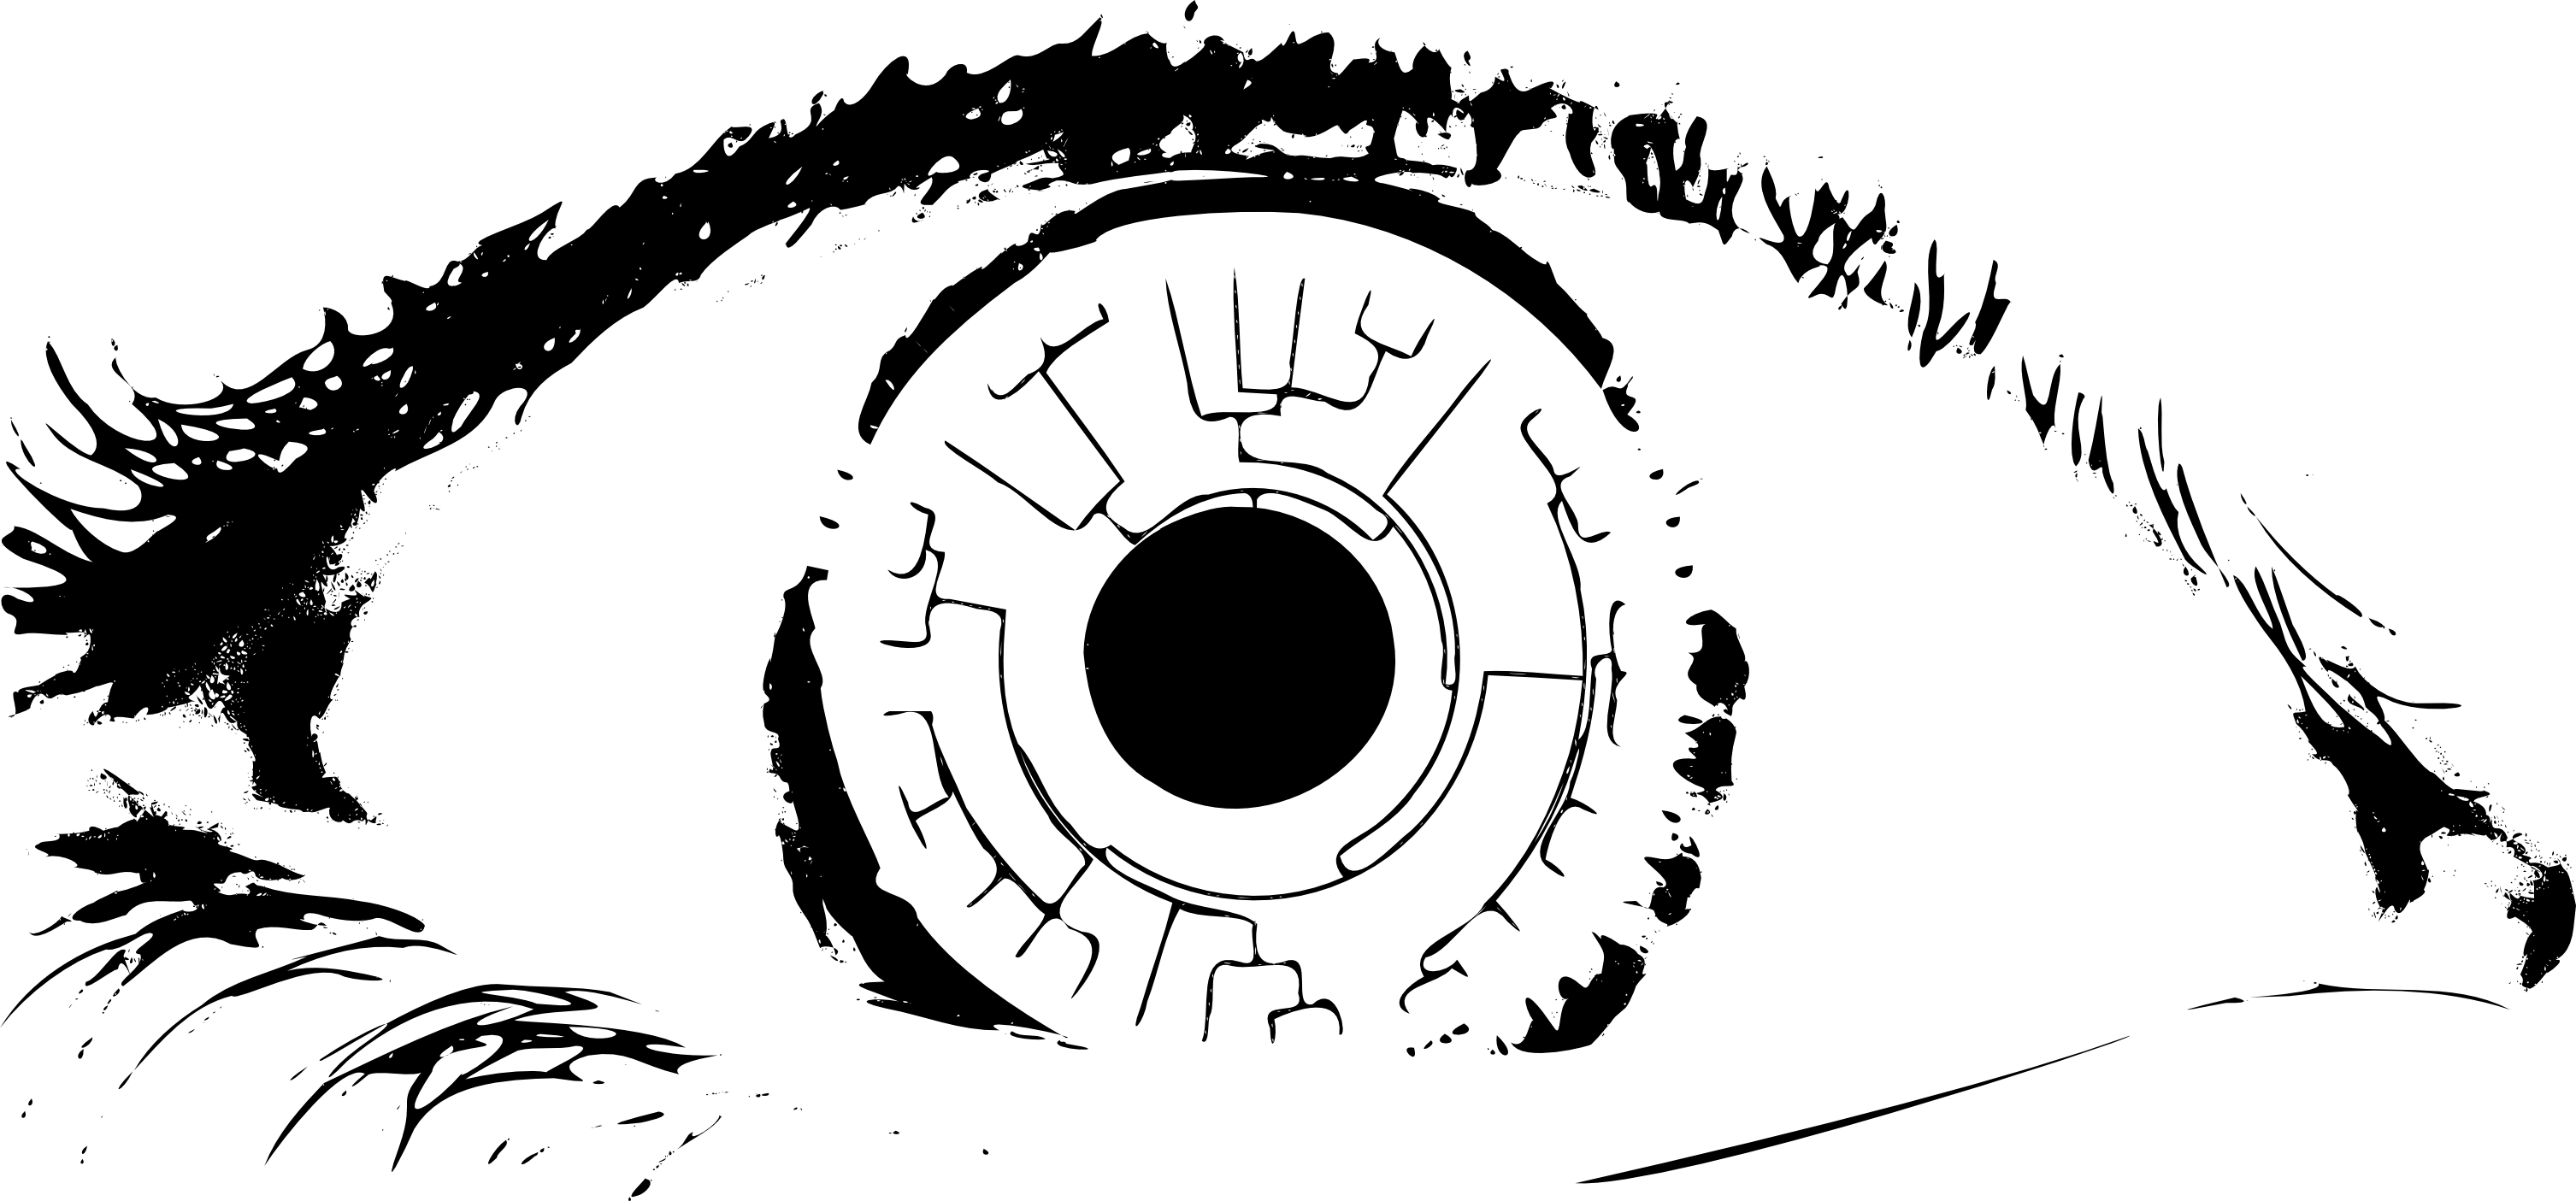
\includegraphics[width=.45\textwidth]{ch2-time/eyepic.png}
\end{figure}

\begin{quoteshrink}
  ``Time is an illusion. Lunchtime doubly so.''

\hfill{Douglas Adams}
\end{quoteshrink}

%%And suddenly I realised that I was no longer driving the car consciously. I was driving it by a %%kind of instinct, only I was in a different dimension.
%% Ayrton Senna


\begin{abstract}
Body size and metabolic rate both fundamentally constrain how species interact with their environment. While many mechanisms leading to these constraints have been explored, their effects on the resolution at which temporal information is perceived have been largely overlooked. The visual system acts as a gateway to the dynamic environment and the relative resolution at which organisms are able to acquire and process visual information is likely to restrict their ability to interact with events around them. As both smaller size and higher metabolic rates should facilitate rapid behavioural responses, we hypothesized that these traits would favour perception of temporal change over finer timescales. Using critical flicker fusion frequency, the lowest frequency of flashing at which a flickering light source is perceived as constant, as a measure of the maximum rate of temporal information processing in the visual system, we carried out a phylogenetic comparative analysis of a wide range of vertebrates that supported this hypothesis. These results have implications for the evolution of signalling systems and predator-prey interactions, and, combined with the strong influence that both body mass and metabolism have on a species' ecological niche, suggest that time perception may constitute an important and overlooked dimension of niche differentiation.
\end{abstract}

\section{Introduction}

All biological systems, from organisms to ecosystems, are shaped by universal constraints. For example, body size and metabolic rate are both known to be important determinants of aspects of organism biology such as life history, energetics and behaviour \citep{brown2004, woodward2005, sibly2012metabolic}. More recently the fundamental role of sensory biology in ecological interactions has gained attention such as research on the limitations imposed on target identification and the scaling allometry of sensory organs \citep{howland2004allometry,cronin2005role,garamszegi2002coevolving}. Such sensory limitations can heavily determine ecological interactions through, for example, predation and mate selection were the abilities of the parties involved to capture, escape or be seduced is dependent on how they perceive their environment (Fig. 1; \citealt{cronin2005role,clark2012field,hornstein2000sexual,stevens2007predator}). While the ability and importance of an organism to perceive the spatial dimensions of its environments are relatively well studied (\citep{cronin2005role,clark2012field}, classic citation on spatial perception Frog targeting?), how they perceive the 4th dimension, time, is less well known.

As the environment is fundamental dynamic in nature the ability to integrate information over timescales is a necessity for any organism interacting within it. The ability to integrate information over shorter timescales, that is, at higher resolutions, is thus a direct limitation on the degree to which it can interact with the environment itself. Furthermore, temporal resolution is also directly linked to the perception of the passage of time itself for humans, in particular when tracking fast moving stimuli \citep{hagura2012ready}. From an evolutionary perspective this leads to a trade-off between the demand for information at high temporal resolution and the costs of its acquisition given the energetic demands associated with increased rates of neural processing in the visual system \citep{laughlin2001energy}. This trade-off is likely to be shaped by various ecological (e.g. mode of predation) and environmental factors (e.g. light levels) as well as intrinsic factors (e.g. morphology) that will ultimately shape an organism's optimal temporal resolution for sensory perception. For example, predators of slow-moving prey may require less temporal resolution than predators that engage in active pursuit of fast-moving prey, such as raptors catching prey during flight.

\begin{figure}[h]
  \centering
  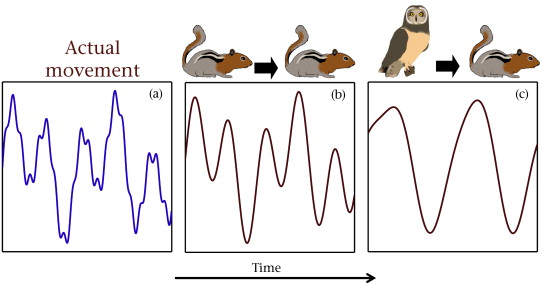
\includegraphics[width=.95\textwidth]{ch2-time/Figure_1.jpg}%Note that this is the path for the folder
  %for chapter 2 that has the Tastes_funny.jpg file within it.
  \caption[Figure 1.]{ The ability of an organism to track a moving object depends on the time integral over which the individual can obtain its information. This is determined by its ability to resolve temporal information. In cases where an animal, such as a ground squirrel, displays complex movement (a), conspecifics may perceive the individual as moving according to a first-order integral of its actual movement owing to its high temporal resolution abilities (b). However a species with lower temporal resolution abilities, such as a short-eared owl, may perceive the motion as an even higher order derivative of the actual motion, meaning information of prey motion at finer temporal scales is not available to it (c).}
  \label{fig:Figure 1.}
\end{figure}


This ability to perceive and react to a dynamic environment is a key behavioural and ecological trait. Ecologically, interaction strengths can be affected by the ability to identify and track fast-moving objects such as prey or mates (Fig. 1; \citealt{land1974chasing, fritsches2005warm}. The necessity of this ability to perceive one's environs accurately is perhaps best demonstrated in cases where temporal resolution is too coarse to allow the observer to follow the motion of a moving target accurately. A stark demonstration of this can be seen in the tiger beetle, Cicindela hudsoni, which, owing to the relatively low temporal resolution of its visual system, must take a stop-start approach in order to recalibrate the position of its prey when hunting \citep{gilbert1997visual}. In humans, the limitations of our temporal perception are apparent when tracking fast-moving objects such as the curving trajectory of a ball in soccer \citep{dessing2010bending} and baseball \citep{bahill2004rising}.

Two intrinsic factors that may shape the costs and benefits of the temporal resolution of the sensory system, in particular with respect to their effects on an individual's ability to interact with the environment on short timescales, are body size and metabolic rate. As larger body sizes decrease manoeuvrability \citep{heglund1988speed,dudley2002mechanisms,biewener2003animal,sato2007stroke,vogel2008modes,hedrick2011damping,watanabe2012slowest} and higher metabolic rates increase both manoeuvrability and the physiological ability to process information \citep{li2008optimal,franz2002temperature}, we hypothesized that smaller organisms and those with higher metabolic rates perceive temporal change on finer timescales.

To quantify the temporal perceptual abilities of a range of species we took advantage of the all or nothing nature of neural firing in the visual system. Owing to this binary firing, temporal resolution must be encoded in terms of discrete units, as biological visual systems must discretize the continuous-time and continuous-space information reaching the retina and then integrate this information over some time period. This "integration time" of visual systems can be quantified using the critical flicker fusion frequency (CFF): the lowest frequency of flashing at which a flickering light source is perceived as constant \citep{d1998can,schwartz2010visual}. As light intensity can increase the number of flashes that can be observed per second, the maximum CFF value, as measured in a response curve of CFF against light intensity \citep{ferry1892persistence,porter1902contributions}, can be used as a proxy for the temporal resolution of the sensory system.

We used CFF to compare the temporal resolution of the visual system in a wide range of vertebrate species including representatives from Mammalia, Reptilia, Aves, Amphibia, Elasmobranchii and Actinopterygii. Using phylogenetic comparative methods and controlling for the light levels each species typically experiences, we tested whether the temporal resolution of the sensory system increases with mass-specific metabolic rate and decreases with body mass.

\section{Methods}
\subsection{Data Collection}
To test our prediction that CFF increases with mass-specific metabolic rate and decreases with body size (when controlling for light levels), we collated data on CFF values of vertebrate species from the literature (Table 1). We only included values from studies that measured CFF using either behavioural or electroretinogram (ERG) procedures. In behavioural studies, CFF is measured through conditional training with the subject trained to respond to a change in its perception of a flashing light \citep{d1998can,rubene2010presence}. For example, \citep{lisney2011behavioural} conducted behavioural tests in domestic chickens, \textit{Gallus gallus}, using choice experiments with flickering and non-flickering stimuli windows with choice of the correct stimulus rewarded with food. This is repeated over a range of light intensities and flicker frequencies until individuals can no longer distinguish between the stimuli. In ERG studies, a direct measurement of the electrical response in the retina in reaction to a flashing light source is used as a measure of CFF \citep{d1998can,schwartz2010visual}. As there may be further processing of temporal information after it reaches the retina that may cause behavioural studies to measure lower CFF values \citep{d1998can}, we included the experimental procedure used to measure CFF as a candidate covariate in our models. We also noted whether each study was a reliable measure of the maximum possible CFF. As maximum CFF is a function of many variables, such as light intensity, and not all studies reported a sufficient range of intensities, their reported CFF may not be the "true maximum" possible. To ensure this did not affect our results we ran an additional analysis that included a term based on this assessment as a categorical covariate as part of our sensitivity analyses (see Appendix).
%changethe end of that to less weak response

We used mean body masses (g) published in the literature and in databases including FishBase \citep{froese2012fishbase} and Animal Diversity Web \citep{myers2006animal} for each species as the measure of body size. For metabolic rates we used mass-specific resting metabolic rate as measured by oxygen consumption through ventilation in studies in which the subjects were fasted prior to the measurement. We converted these values to W/g using the conversion of 20 J/ml of oxygen consumption \citep{makarieva2008mean} to allow comparison among species. For ram-ventilation species (which require constant movement to force fluid over the respiratory organs), such as sharks and tuna, the resting metabolic rate was taken as the fitted line of oxygen consumption with swimming speed extrapolated to the intercept (swimming speed = 0 m/s; Table 1). To account for the possible effect of metabolic rate measured at different temperatures in ectothermic species, metabolic rate values were corrected to 20 $^{\circ}$C using Q10 values, i.e. the fold change in metabolic rate over a temperature change of 10 $^{\circ}$C, for reptiles, amphibians and fish \citep{white2006scaling}. These corrections gave values of temperature-corrected mass-specific resting metabolic rates (qWg), for each species. Although body mass and mass-specific metabolic rate are expected to be correlated according to an exponent of 0.25 \citep{brown2004, sibly2012metabolic} (Brown et al., 2004 and Sibly et al., 2012), we included both terms as recommended by \citep{freckleton2009seven} instead of using residuals from a regression of body mass against mass-specific metabolic rate.

As there is a trade-off between sensitivity and movement perception owing to the requirement of longer integration times in low light conditions \citep{tansley1965vision}, as is seen in the different light response dynamics of rods and cones \citep{rubene2010presence}, we included light levels within our analyses as a categorical variable based on the light conditions experienced by the species during normal activity (i.e. foraging). Species were categorized as inhabiting either high or low light conditions with diurnal terrestrial and nonturbid aquatic species coded as inhabiting high light level environments and nocturnal species coded as inhabiting low light levels. As the light levels of species that inhabit turbid waters are typically orders of magnitude lower than typical daylight levels (40-1000 lx; \citealt{ali1985vision,palmer2010art,kreysing2012photonic} and the harp seal, Pagophilus groenlandicus, regularly forages at depths greater than 200m \citep{folkow2004distribution} where light levels are comparable to nocturnal light levels (Palmer and Grant 2010), we categorized these species as inhabiting low light level environments.


\begin{figure}[h!]
  \centering
  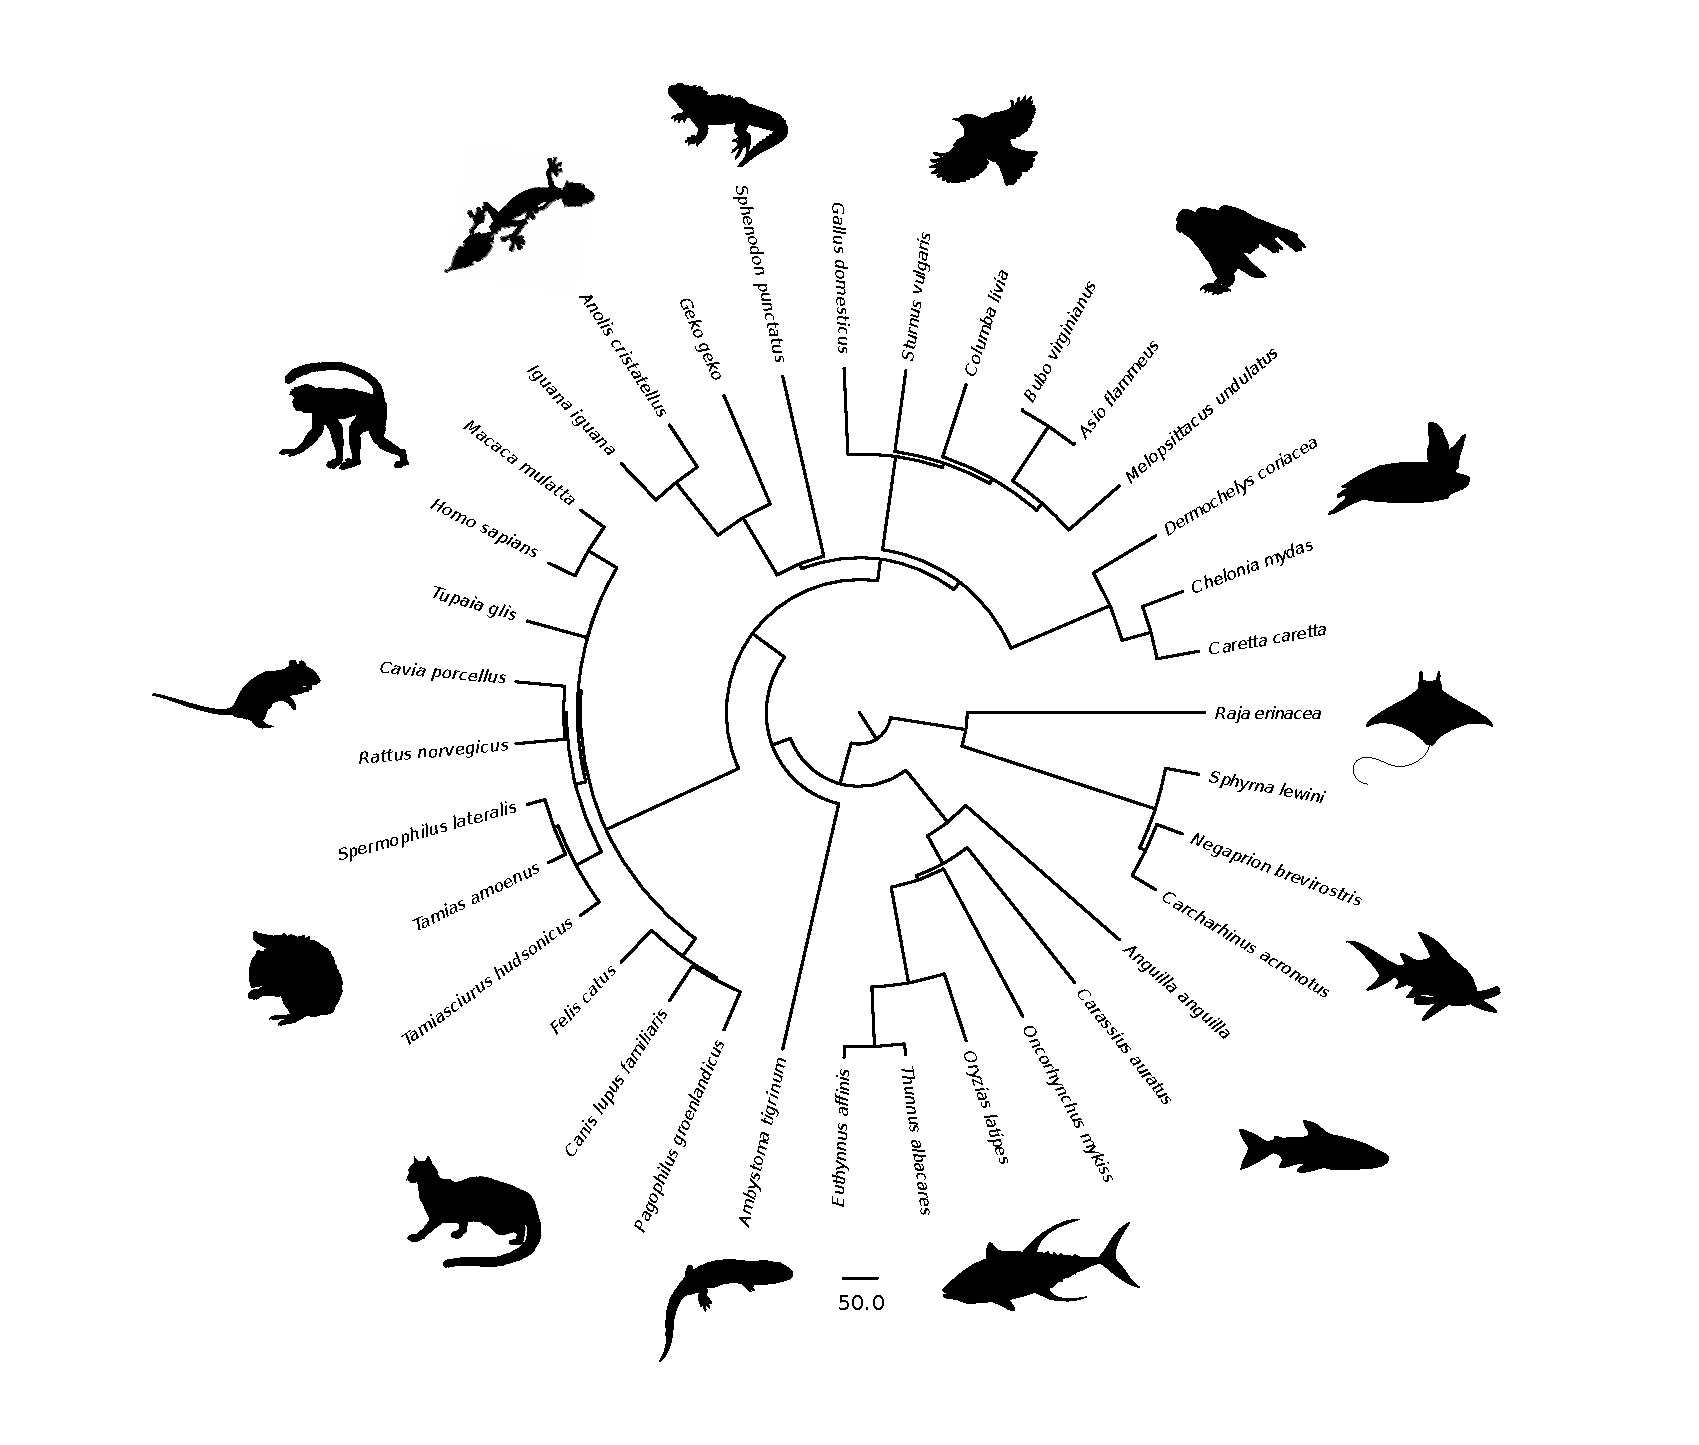
\includegraphics[width=.95\textwidth]{ch2-time/phylofig.pdf}%Note that this is the path for the folder
  %for chapter 2 that has the Tastes_funny.jpg file within it.
  \caption[Figure 2.]{ Composite tree of the study species.}
  \label{fig:Figure 2.}
\end{figure}


To correct for the phylogenetic nonindependence of species we constructed a composite tree of the study species using published molecular phylogenies and divergence times from various sources \citep{schoch1985preliminary,janossy2011pleistocene,mercer2003effects,hedges2006timetree,wiens2006does,benton2007paleontological,murphy2007using,brown2008strong,li2008optimal,naro2008evolutionary,albert2009effect,lim2010phylogeny,little2010evolutionary,perelman2011molecular} (Schoch, 1985,; see the Appendix and Fig. A1). In instances in which a divergence time was not available for two species we used the conservatively estimated date of first appearance as the divergence time taken from the Paleobiology Database \citep{alroy2008phanerozoic}.



As ectotherm metabolic rates vary with temperature, we performed a sensitivity analysis to test the effect of the temperature to which qWg was corrected to by rerunning the main analysis with qWg corrected to both 5 °C and 35 °C (see Appendix). We also carried out a supplemental analysis on a more restricted data set for species with available brain mass data to test for any possible effects of sensory tissue on maximum CFF values (see Appendix).

In total we collected data on maximum CFF, body mass, qWg and light environments for 34 species across the vertebrate classes Elasmobranchii, Actinopterygii, Aves, Amphibia, Reptilia and Mammalia, with further data on brain mass for 28 of these species (Table 1).

\subsection{Statistical Analyses}
To test our hypothesis we used a phylogenetic generalized least-squared approach (PGLS) using the caper package \citep{orme2011caper} in R version 2.14.2 \citep{RCran}. The PGLS approach is based on standard generalized least-squared models while also accounting for the nonindependence in the data caused by species' phylogenetic relationships by incorporating it through the error term structure \citep{pagel1999inferring,rohlf2001comparative}. This error term consists of a matrix of expected trait covariances calculated using the maximum likelihood estimate of lambda (), a multiplier of the off-diagonal elements of a phylogenetic variance–covariance matrix that best fits the data. When the data are structured according to a Brownian motion of trait evolution, lambda = 1, whereas when the data have no phylogenetic dependency, then lambda = 0 \citep{pagel1999inferring}.

We ran PGLS models with maximum CFF as the response variable, and all combinations of the following explanatory variables: body mass, qWg, light level (high, low) and experimental procedure (ERG, behavioural) with brain mass and methodological optimality included in the sensitivity analysis (see Appendix). We did not include interactions, as there was no a priori reason to include them. We used the Akaike information criterion (AIC), which penalizes extra effective parameters to avoid overparameterized models, to select the minimum adequate model \citep{burnham2002model}.


\begin{table}[h!]
  \caption[Table 1.]{Data used in analysis}
  \label{tbl:Table 1.}
  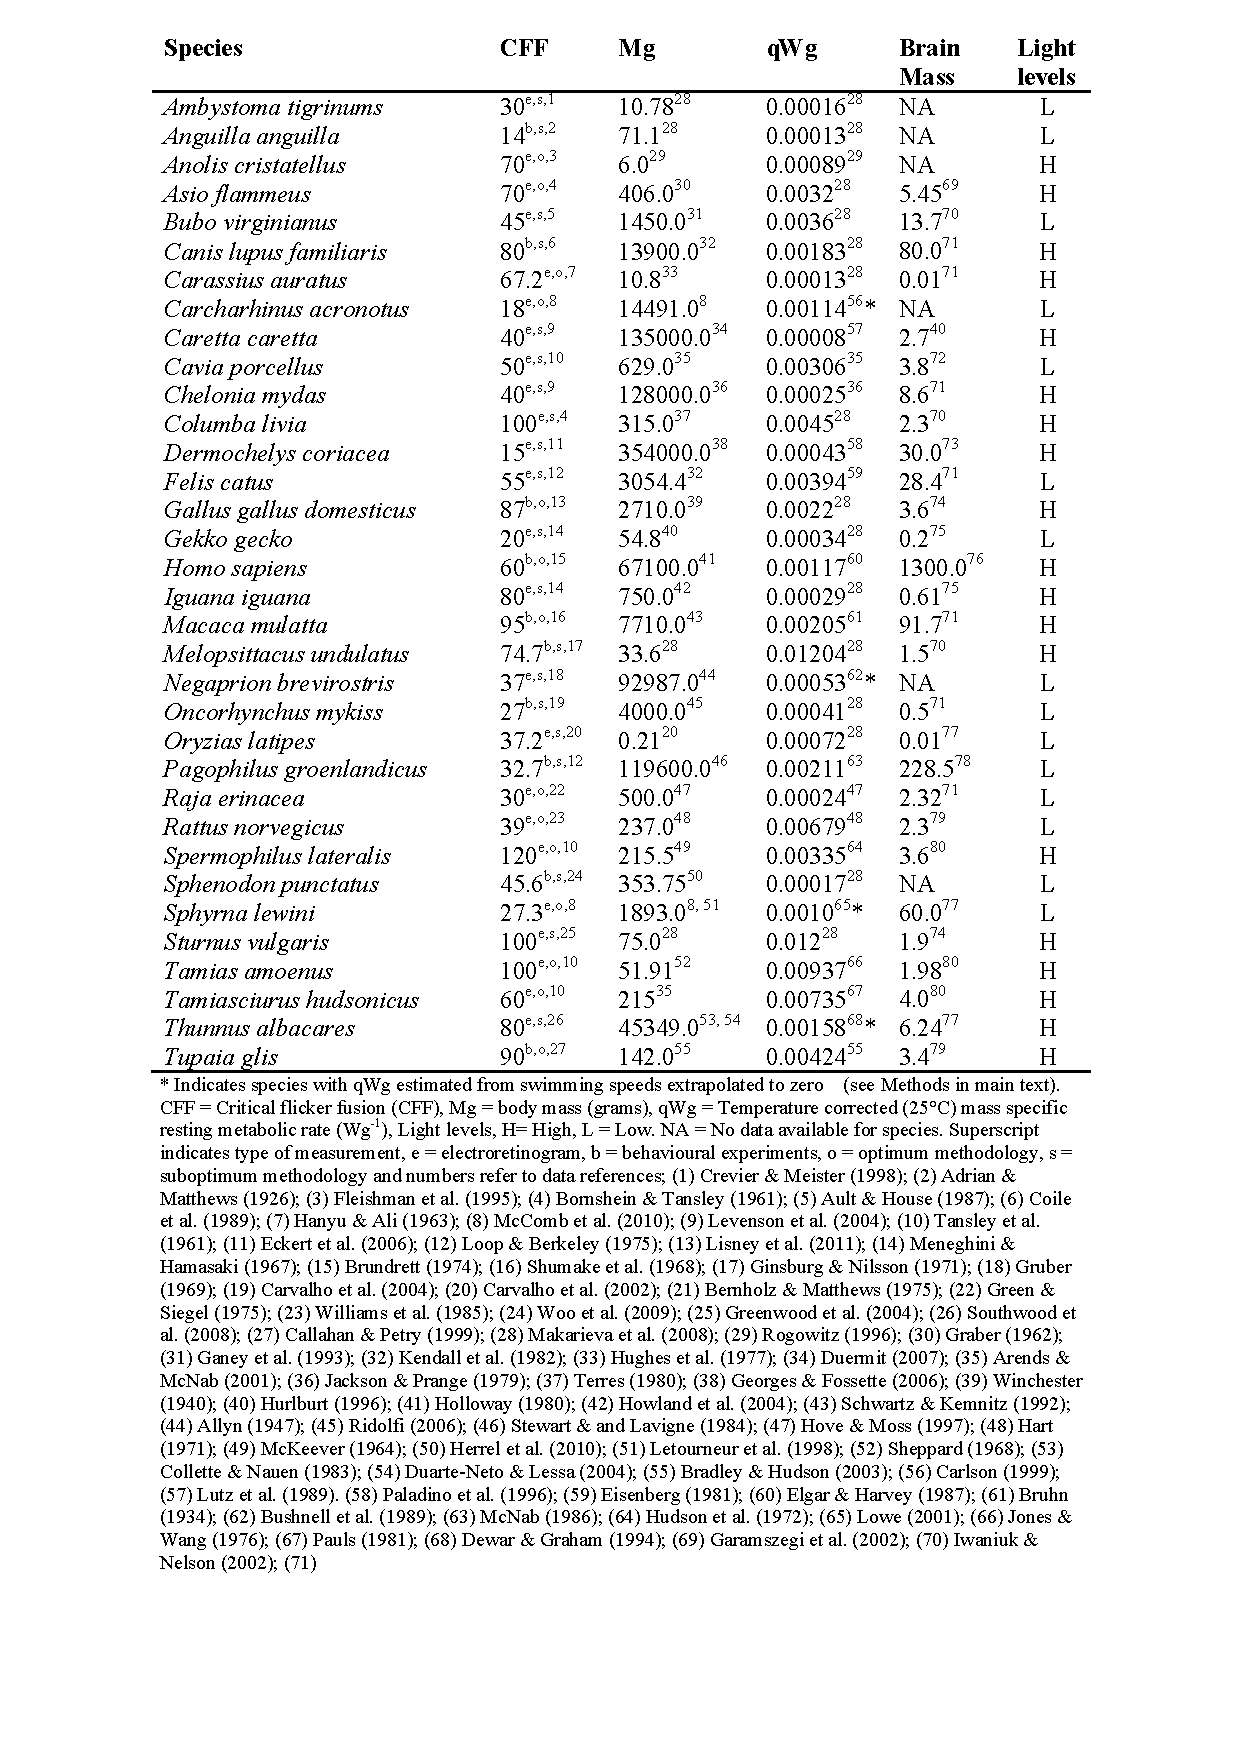
\includegraphics[width=\linewidth]{ch2-time/Table_1}
\end{table}


\section{Results}
The most parsimonious model (based on AIC) explaining variation in maximum CFF among vertebrates included the terms body mass, temperature-corrected mass-specific resting metabolic rate (qWg) and light level (Table 2, Tables A1 and A5 in the Appendix). The second most parsimonious model, which fell within two AIC values of the most parsimonious model, retained all tested variables (Table 2). Body mass had a negative effect on the temporal resolution of the sensory system (Table 2, Fig. 2a, Fig. A2 in the Appendix), with a change in body mass of approximately 10 kg resulting in a reduction in CFF of 2 Hz. The metabolic rate of organisms, after correcting for mass, was positively associated with CFF while low environmental light levels were associated with an overall reduction in CFF (Table 2, Fig. 2b, Fig. A2 in the Appendix). Phylogeny was found to have a minimal effect on the resulting models (λ = 0, Table 2) and experimental type was not correlated with CFF (Table 2). Thus, according to our model, small animals with high mass-specific metabolic rates in high light environments possessed the highest maximum CFF and hence greatest ability to perceive temporally dynamic visual information. Conversely, large animals with low mass-specific metabolic rates in low light environments had the lowest CFF.


\begin{table}[h!]
  \centering
    \caption[Table 2.]{Coefficients of the model with all factors included. Mg = body mass (grams), qWg = Temperature corrected mass-specific resting metabolic rate Wg-1, Light.l (low) = effect of low light levels on CFF in comparison to high light levels, exp = effect of experimental type (ERG = electroretinogram) in comparison to behavior based CFF measures.}

\begin{tabular}{*5l}    \toprule
\emph{Variable} & \emph{Estimate} & \emph{S.E} & \emph{t-value}&  \emph{P-value}\\\midrule
Intercept    & 141.48  & 15.15  & 9.34  &  {\ensuremath{4^{-10}}}\\ 
Mg & -4.40 & 2.01 & -2.18 & 0.038\\
qWg & 16.89 & 4.31 & 3.92 & {\ensuremath{5^{-4}}}\\
Light levels (low) & -37.74 & 5.94 & -6.36 & {\ensuremath{7^{-7}}}\\
Measurement type (exp) & -3.66 & 6.24 & -0.59 & 0.56\\
Data quality (high) & -3.86 & 6.14 & -0.63 & 0.53\\
 &  & & & \\
 & Mode & Lower 95\% C.I & Upper 95\% C.I\\ 
Lambda  (Low) & 0 & 0 & 0.34 &\\
&  &  &  &{\ensuremath{R^2}= 0.69}\\\bottomrule
 \hline
\end{tabular}
  \label{tbl:Table 2.}
\end{table}


These results were robust to our sensitivity analysis on both the temperature used to correct ectotherms qWg (taken as 25 °C in the main models above; see Methods) and the optimality of study methodology for measuring maximum CFF, with the best models in both sensitivity analyses (based on AIC) including the same terms and trends as found in the main analysis (Tables A2, A3, A5, A6, A7 and A9 in the Appendix). We also found that including brain mass in a restricted data set of 28 species for which brain mass was available did not change the effect of the explanatory variables light levels, qWg and body mass on maximum CFF (Tables A4 and A8 in the Appendix).


\begin{figure}[h!]
  \centering
  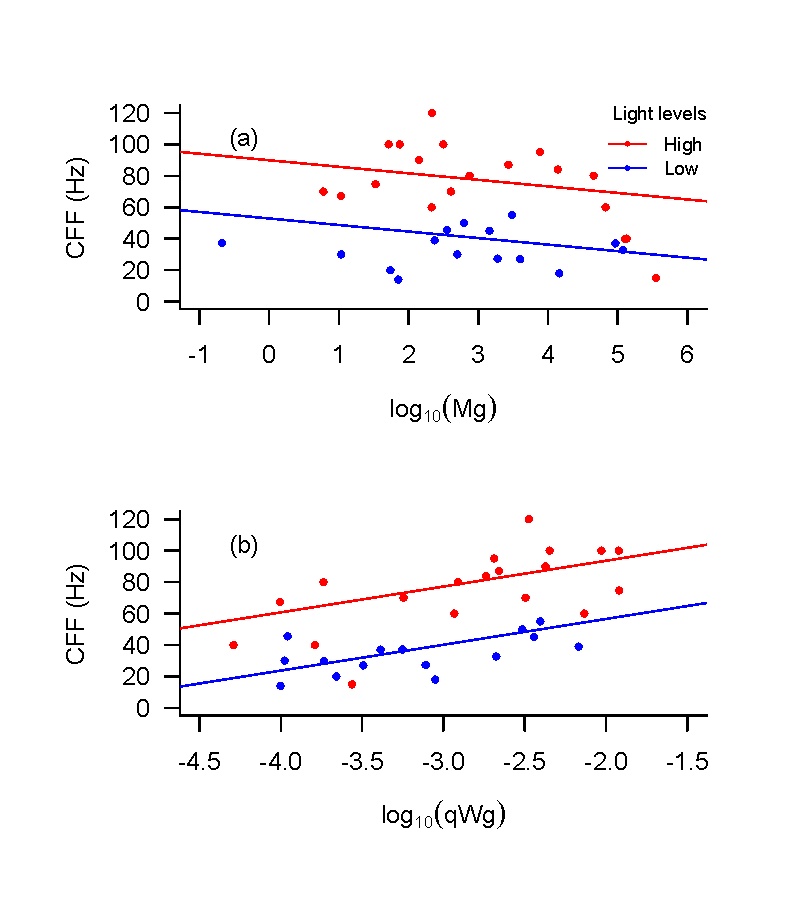
\includegraphics[width=.95\textwidth]{ch2-time/Figure_2}%Note that this is the path for the folder
  %for chapter 2 that has the Tastes_funny.jpg file within it.
  \caption[Figure 3.]{ The effect of  log body mass, light levels and log temperature corrected mass-specific resting metabolic rate (qWg) on critical flicker fusion frequency (CFF). The minimal adequate model (Results) indicates CFF increases with log qWg but decreases with body mass. Low light levels (blue) are associated with low CFF values in comparison to high light levels (red).}
  \label{fig:Figure 3.}
\end{figure}


\section{Discussion}
Many of the interspecific and intraspecific interactions that shape species' behaviour and ecology rely on the ability of organisms to process high temporal resolution sensory information. Our results show that, while there is considerable variability in the ability to resolve temporally dynamic visual information across vertebrates, body mass and metabolic rate act as important general constraints on this ability. This is the first study to indicate a general trend in the ability of vertebrates to resolve temporal information; previous studies have generally focused on specific cases of sensory adaptations \citep{fritsches2005warm} and particular environments \citep{frank1999comparative,frank2012light}, hence focusing on the particular ecological context of each adaptation or environment. Our findings illustrate the relationship between both physiology and the effects of body mass on the ability to resolve temporal features of the environment on fine timescales, hence linking sensory adaptations to fundamental constraints and trade-offs imposed on all organisms.

\cite{autrum1958electrophysiological} hypothesis, that the response dynamics of the retina should be shaped by the organism's particular ecology, predicts that organisms that demand fast visual systems will acquire adaptations increasing CFF values, and hence temporal resolution. This can be achieved through alterations to the rate of neuron firing, a fundamental limit to the rate of information transfer, through the provision of energy \citep{laughlin2001energy} or changes in the physiological environment. For example, blowflies \citep{tatler2000temperature} and predatory swordfish \citep{fritsches2005warm} both use specialised heating tissues that increase the temperature, and hence the metabolic rate, in their visual systems, which in turn up-regulates their CFF. Similar adaptations are also seen across species of large, fast-swimming predatory billfish \citep{carey1982brain} and Lamnidae sharks \citep{block1985warm}. Physiological adaptations for high-resolution motion detection are also found within specific areas of the retina in some flies, commonly referred to as the "love spot", which allow them to identify female flight patterns accurately and thus detect mates \citep{land1974chasing}.

In a broader context, it might be expected that manoeuvrability, a vital component of an individual's ability to respond to the environment, may be one of the main factors determining whether it is necessary to invest in costly temporal information processing. Manoeuvrability, as defined by the ability to change body position or orientation, generally scales negatively with body mass. This negative scaling emerges primarily through the increased inertia and decreased limb stroke rate associated with large body size in both aquatic and volant species \citep{dudley2002mechanisms,sato2007stroke,vogel2008modes,hedrick2011damping,watanabe2012slowest}, while in terrestrial species changes in gait posture that redistribute weight across the limbs can explain such reduced manoeuvrability with body mass \citep{heglund1988speed,biewener2003animal}. These arguments show that, owing to the laws of physics, larger animals physically respond less quickly to a stimulus. Hence we expect selection against costly investment in sensory systems with unnecessarily high temporal resolution in large animals, as information on such timescales can no longer be utilized effectively. This may explain why larger vertebrates, along with those with low metabolic rates, had lower temporal resolution in our study. This idea is also supported by research showing that faster and more manoeuvrable fly species have higher temporal resolutions \citep{laughlin1993fast} and that less manoeuvrable scavenger crabs display slower response dynamics than deeper living predatory species which are likely to have more active lifestyles \citep{frank2012light}.


While many species have evolved adaptations to overcome sensory limitations most species in our results conform to a general scaling in their temporal ability. Hence while body size and metabolic rate are known to good proxies to the rate which individuals can interact with the environment we show that this proxy also extends towards perceptual abilities. Hence while a individual may be theoretically capable of interacting with another individual, its inability to track its movement or fully process a signal may practically excuse it form the interaction.


The effects of body size and metabolic rate on temporal resolution and the presence of sensory adaptations, as discussed above, also point towards an interesting dimension of niche space. Disparity in size and metabolic rate among species within an ecological setting may select for particular sets of adaptations creating a diverse set of sensory systems and interactions. In such a system, species might occupy the same spatial and temporal niche, but could be separated owing to differential responsiveness to environmental signals and cues as a result of having evolved divergent signalling systems along a dimension represented by temporal resolution. For example, it seems at least theoretically possible to encode information in high-frequency signals that can be detected by intended receivers such as conspecifics but that are not susceptible to "eavesdropping" by (generally larger) predators. Ecological systems in which this may be apparent include deep-sea systems where visual signalling is an important determinant of the ability of organisms to interact, and where bioluminescence flashing over wide frequency ranges is ubiquitous \citep{haddock2005bioluminescent,widder2010bioluminescence}.


Overall our results show that not only are body size and metabolic rate good proxies for the rate of biological interactions they are good proxies for the ability to perceive such interactions. While interaction rates are strongly coupled with the spatial dimensionality of the environment and searching rates associated with them \citep{pawar2012dimensionality} the temporal dimension in which an individual resides will also strongly influence its ability to interact with that environment. The generality of these findings suggest that temporal resolution may play a much more important role in sensory ecology than previously indicated, in particular because of its universal effects relating to body size. Further investigations into both the underlying mechanisms of these findings and their importance to ecological functioning are needed.


\bibliographystyle{PLoS-Biology}
\bibliography{bibfile}

